%\documentclass[12pt,a4paper]{article}
\documentclass[12pt,letter]{article}
%% Aquí empieza el preámbulo

\usepackage{amsmath}
%%% Paquetes a utilizar
\usepackage[spanish]{babel}
% Para insertar imágenes
\usepackage{graphicx}
% Para multiples imágenes en la misma figura
\usepackage{caption}
\usepackage{subcaption}
\graphicspath{{./imagenes/}}

\usepackage{minted}

%%% Metadatos del documento
\title{Título del documento (artículo)}
\author{Fulanito deTal, Fulanita X} 
\date{1 de mayo de 2026}



%% Aquí termina el preámbulo
\begin{document}
\maketitle

\begin{abstract}
          
Latex es una aplicación para preparar documentos aplicando un
lenguaje de marcado. Permite producir textos escritos de alta calidad,
especializado en composición de expresiones de matemáticas, física,
fórmulas, desde una fórmula estándar para uso general hasta artículos
científicos, libros, informes y tesis. El propósito de este ejemplo es
que sirva como una plantilla de \LaTeX para generar documentos útiles
para hacer reportes de asignaturas científicas. Esto es, que la
estructura de este documento replica la estructura del método
científico a través de las secciones de: {\em Introducción, Métodos,
  Resultados, Discusión y Conclusiones} y soporta el uso de figuras,
tablas, gráficas y referencias bibliográficas.  


\vspace{1cm}
\noindent Palabras clave: \texttt{keyword1, keyword2, keyword3, keyword4}.

\end{abstract}  
% Esto es un comentario
\section{Introducción}

La sección de introducción en un reporte científico es la parte
inicial que presenta el problema de estudio, el estado del arte, la
brecha en el conocimiento y el objetivo de la investigación,
estableciendo el contexto y justificando su relevancia.
Responde a las preguntas: ¿Qué?, ¿Por qué? y ¿Para qué?.

En LaTeX, una sección se emplea para comenzar una parte
sustancial del documento. Proporciona un título descriptivo impreso,
y, según la clase del documento, una numeración automática (como 1.,
2.A o incluso "Sección Práctica"), y suele añadir una entrada
automática en la tabla de contenidos (ToC). También genera un salto de
página o de columna si la clase de documento lo define así.

\section{Métodos}

La sección de métodos en un informe científico describe cómo se
realizó el estudio o el experimento. Debe describir precisamente cómo
se realizaron las observaciones, experimentos y análisis. La finalidad
de esto es que se pueda replicar por otras personas y corroborar los
resultados obtenidos.

Por ejemplo en la figura \ref{img:graph}.

\begin{figure}[h]
  \centering 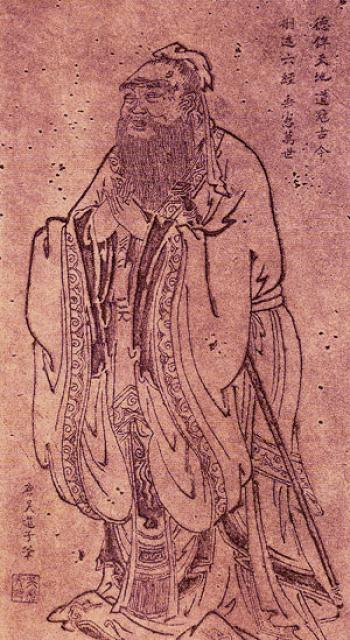
\includegraphics[width=.4\linewidth]{confucius.jpg}
  \caption{Descripción de la imágen. En este caso, un retrato de
    Confucio tomado de la Wikipedia.}
  \label{img:graph}
\end{figure}


\subsection{Esto es el título de una subsección}
\label{sec:subsección}
Una subsección en LaTeX se define mediante el comando
\texttt{subsection\{\}}. Este comando genera automáticamente un número de subsección y da formato al título fomentando la estructura lógica del documento. Sitúa el texto indicado en la clase del documento y permite hacer referencias mediante \texttt{label\{\}}.  

Sigamos con las imágenes. Podemos hacer una tabla de imágenes
utilizando el paquete \texttt{subcaption} o \texttt{subfig}.
Por ejemplo, para insertar una imagen con 2x2 imágenes (es decir, 4
subfiguras). En la subfigura \ref{img:confucio}, se ve a confucio, en
la figura \ref{img:laotze}, se puede ver a Lao-Tze, etc..

\begin{figure}[h]
    \centering
    \begin{subfigure}[b]{0.24\linewidth}
        \centering
        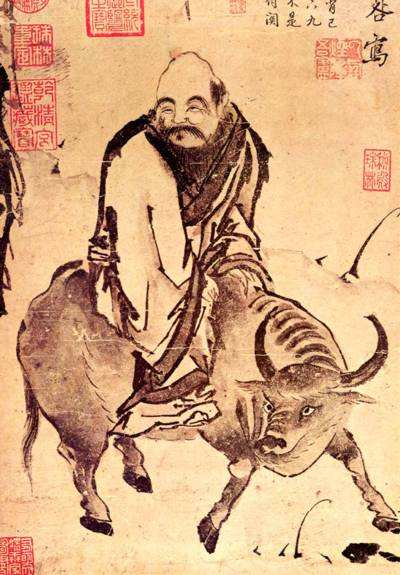
\includegraphics[width=\linewidth, height=5cm]{Laozi.jpg}  % Replace with actual image name
        \caption{Retrato de Lao-Tse (Wikipedia)}
        \label{img:laotze}
    \end{subfigure}
    %\hfill
    \begin{subfigure}[b]{0.24\linewidth}
        \centering
        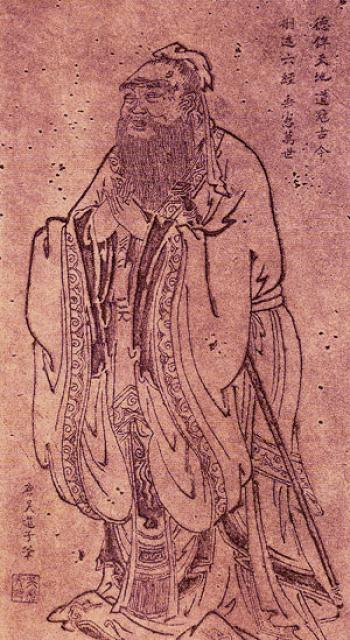
\includegraphics[width=\linewidth , height=5cm]{confucius.jpg}  % Replace with actual image name
        \caption{Retrato de Confucio}
        \label{img:confucio}
    \end{subfigure}
    \vspace{1.0\baselineskip}
    % Add second row here for 2x2 layout
    \begin{subfigure}[b]{0.24\linewidth}
        \centering
        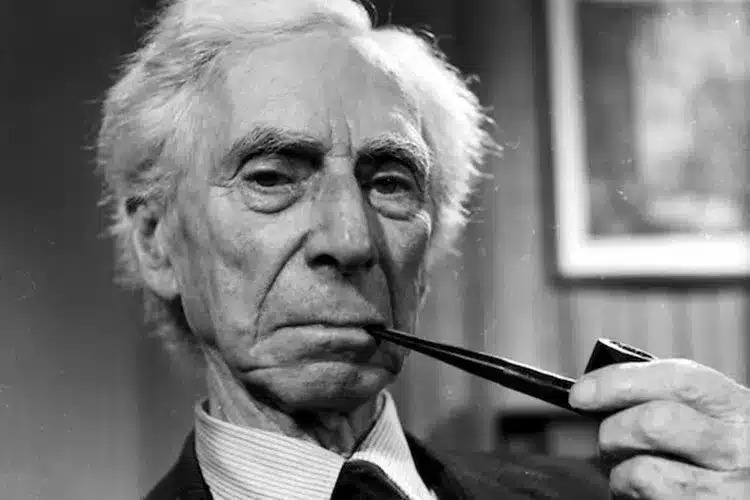
\includegraphics[width=\linewidth, height=5cm]{russel.jpg}  % Replace with actual image name
        \caption{Retrato de Russel}
        \label{img:russel}
    \end{subfigure}
    %\hfill
    \begin{subfigure}[b]{0.24\linewidth}
        \centering
        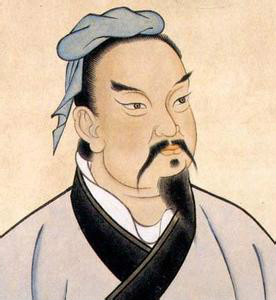
\includegraphics[width=\linewidth, height=5cm]{suntzu.jpg}  % Replace with actual image name
        \caption{Retrato de Suntzu}
        \label{img:suntzu}
    \end{subfigure}
    \caption{Una muestra de cuatro retratos}
    \label{img:retratos}
\end{figure}


\subsection{Formato de Texto}
Para hacer listas:
\begin{itemize}
  \item Texto en \textbf{Negritas}
  \item Texto en {\em Cursiva}
  \item Texto \texttt{Máquina de escribir}
\end{itemize}        

\subsection{Tablas}
Las tablas o cuadros no sirven para representar relaciones entre datos.




\begin{table}
  \label{tab:ejemplo1}
  \caption{Este es un ejemplo de un curso con calificaciones.}
  \centering
\begin{tabular}{|c c c c c c|}
  \hline
  \textbf{Alumno} & Ex 1 & Ex 2 & Ex 3 & Ex 4 &                                                                                 \textbf{Promedio} \\
  \hline
Ana Pérez & 7.5 & 8.0 & 9.0 & 7.0 & 7.9 
\\
Juan López & 6.0 & 7.0 & 8.5 & 6.5 & 7.0 
\\
María García & 9.0 & 9.5 & 8.9 & 8.5 & 9.0 
\\
Carlos Ruiz & 8.0 & 8.5 & 8.0 & 7.5 & 8.0
\\
\hline
\end{tabular}
\end{table}  

\subsection{Ejemplo para mostrar código}

Para mostrar código podemos usar el ambiente 'Verbatim'.

\begin{minted}{python}
def fibonacci(n):
    fib_secuence = []
    a, b = 0, 1
    
    while len(fib_secuence) < n:
        fib_secuence.append(a)
        a, b = b, a + b
    return fib_secuence

n = int(input("Manual Sequence n value? \n"))
print("Fibonacci sequence:")
fibonacci_seq = fibonacci(n)
print(fibonacci_seq)
\end{minted} 

Esta palabra es {\large large} pero esta es más {\em Grande}

  \section{Ecuaciones y símbolos matemáticos}

  Se pueden poner en la misma línea con \$ ecuacion entre signo de peso\$ por ejemplo:
  $f(x) = x^{23}_{i,j} + xy + \epsilon$.
  Con dos signos de peso (\$\$) lo hace en línea separada.

  $$ f(x) = \log(x^n) + \exp^{\alpha_ix}$$

  \subsection{Ambiente para ecuaciones}
  También hay un ambiente para ecuaciones para poner referencias e
  índices.

La función de densidad de probabilidad de una distribución gaussiana (normal) con media $\mu$ y varianza $\sigma^2$ es:

\begin{equation} \label{eq1}
\begin{split}
A & = \frac{\pi r^2}{2} \\
 & = \frac{1}{2} \pi r^2 \\
 & = \frac{1}{2} \pi r^2 \\
 & = \frac{1}{2} \pi r^2 \\
 & = \frac{1}{2} \pi r^2 \\
 & = \frac{1}{2} \pi r^2 \\
 & = \frac{1}{2} \pi r^2 \\
 & = \frac{1}{2} \pi r^2 \\
 & = \frac{1}{2} \pi r^2 
\end{split}
\caption{Leyenda de la ecuación}
\end{equation}
  
  Tell me, Muse, of that man, so ready at need, who wandered far and
wide, after he had sacked the sacred citadel of Troy, and many were the
men whose towns he saw and whose mind he learnt, yea, and many the woes
he suffered in his heart on the deep, striving to win his own life and}
the return of his company. Nay, but even so he saved not his company,
though he desired it sore. For through the blindness of their own
hearts they perished, fools, who devoured the oxen of Helios Hyperion:
but the god took from them their day of returning. Of these things,
goddess, daughter of Zeus, whencesoever thou hast heard thereof,
declare thou even unto us.

\subsubsection{Subsubsección}
    \noindent Now all the rest, as many as fled from sheer destruction, were at
    home, and had escaped both war and sea, but Odysseus only, craving
    for his wife and for his homeward path, the lady nymph Calypso
    held, that fair goddess, in her hollow caves, longing to have him
    for her lord. But when now the year had come in the courses of the
    seasons, wherein the gods had ordained that he should return home
    to Ithaca, not even there was he quit of labours, not even among
    his own; but all the gods had pity on him save Poseidon, who raged
    continually against godlike Odysseus, till he came to his own
    country. Howbeit Poseidon had now departed for the distant
    Ethiopians, the Ethiopians that are sundered in twain, the
    uttermost of men, abiding some where Hyperion sinks and some where
    he rises.

    \paragraph{Párrafo}
    There he looked to receive his hecatomb of bulls and
    rams, there he made merry sitting at the feast, but the other gods
    were gathered in the halls of Olympian Zeus. Then among them the
    father of men and gods began to speak, for he bethought him in his
    heart of noble Aegisthus, whom the son of Agamemnon, far-famed
    Orestes, slew.
    
    \subparagraph{Subpárrafo} Thinking upon him he spake out among the Immortals:
    ‘Lo you now, how vainly mortal men do blame the gods! For of us
    they say comes evil, whereas they even of themselves, through the
    blindness of their own hearts, have sorrows beyond that which is
    ordained. Even as of late Aegisthus, beyond that which was
    ordained, took to him the wedded wife of the son of Atreus, and
    killed her lord on his return, and that with sheer doom before his
    eyes, since we had warned him by the embassy of Hermes the
    keen-sighted, the slayer of Argos, that he should neither kill the
    man, nor woo his wife. For the son of Atreus shall be avenged at
    the hand of Orestes, so soon as he shall come to man’s estate and
    long for his own country. So spake Hermes, yet he prevailed not on
    the heart of Aegisthus, for all his good will; but now hath he paid
    one price for all.’
    \paragraph{}
    And the goddess, grey-eyed Athene, answered him, saying: ‘O father,
    our father Cronides, throned in the highest; that man assuredly
    lies in a death that is his due; so perish likewise all who work
    such deeds! But my heart is rent for wise Odysseus, the hapless
    one, who far from his friends this long while suffereth affliction
    in a sea-girt isle, where is the navel of the sea, a woodland isle,
    and therein a goddess hath her habitation, the daughter of the
    wizard Atlas, who knows the depths of every sea, and himself
    upholds the tall pillars which keep earth and sky asunder. His
    daughter it is that holds the hapless man in sorrow: and ever with
    soft and guileful tales she is wooing him to forgetfulness of
    Ithaca. But Odysseus yearning to see if it were but the smoke leap
    upwards from his own land, hath a desire to die. As for thee, thine
    heart regardeth it not at all, Olympian! What! Did not Odysseus by
    the ships of the Argives make thee free offering of sacrifice in
    the wide Trojan land? Wherefore wast thou then so wroth with him, O
    Zeus?’


The “Odyssey” (as every one knows) abounds in passages borrowed from
the “Iliad”; I had wished to print these in a slightly different type,
with marginal references to the “Iliad,” and had marked them to this
end in my MS. I found, however, that the translation would be thus
hopelessly scholasticised, and abandoned my intention. I would
nevertheless urge on those who have the management of our University
presses, that they would render a great service to students if they
would publish a Greek text of the “Odyssey” with the Iliadic passages
printed in a different type, and with marginal references. I have given
the British Museum a copy of the “Odyssey” with the Iliadic passages
underlined and referred to in MS.; I have also given an “Iliad” marked
with all the Odyssean passages, and their references; but copies of
both the “Iliad” and “Odyssey” so marked ought to be within easy reach
of all students.

Any one who at the present day discusses the questions that have arisen
round the “Iliad” since Wolf’s time, without keeping it well before his
reader’s mind that the “Odyssey” was demonstrably written from one
single neighbourhood, and hence (even though nothing else pointed to
this conclusion) presumably by one person only—that it was written
certainly before 750, and in all probability before 1000 B.C.—that the
writer of this very early poem was demonstrably familiar with the
“Iliad” as we now have it, borrowing as freely from those books whose
genuineness has been most impugned, as from those which are admitted to
be by Homer—any one who fails to keep these points before his readers,
is hardly dealing equitably by them. Any one on the other hand, who
will mark his “Iliad” and his “Odyssey” from the copies in the British
Museum above referred to, and who will draw the only inference that
common sense can draw from the presence of so many identical passages
in both poems, will, I believe, find no difficulty in assigning their
proper value to a large number of books here and on the Continent that
at present enjoy considerable reputations. Furthermore, and this
perhaps is an advantage better worth securing, he will find that many
puzzles of the “Odyssey” cease to puzzle him on the discovery that they
arise from over-saturation with the “Iliad.”

Other difficulties will also disappear as soon as the development of
the poem in the writer’s mind is understood. I have dealt with this at
some length in pp. 251-261 of “The Authoress of the Odyssey”. Briefly,
the “Odyssey” consists of two distinct poems: (1) The Return of
Ulysses, which alone the Muse is asked to sing in the opening lines of
the poem. This poem includes the Phaeacian episode, and the account of
Ulysses’ adventures as told by himself in Books ix.-xii. It consists of
lines 1-79 (roughly) of Book i., of line 28 of Book v., and thence
without intermission to the middle of line 187 of Book xiii., at which
point the original scheme was abandoned.

(2) The story of Penelope and the suitors, with the episode of
Telemachus’ voyage to Pylos. This poem begins with line 80 (roughly) of
Book i., is continued to the end of Book iv., and not resumed till
Ulysses wakes in the middle of line 187, Book xiii., from whence it
continues to the end of Book xxiv.

In “The Authoress of the Odyssey”, I wrote:

the introduction of lines xi., 115-137 and of line ix., 535, with the
writing a new council of the gods at the beginning of Book v., to take
the place of the one that was removed to Book i., 1-79, were the only
things that were done to give even a semblance of unity to the old
scheme and the new, and to conceal the fact that the Muse, after being
asked to sing of one subject, spend two-thirds of her time in singing a
very different one, with a climax for which no-one has asked her. For
roughly the Return occupies eight Books, and Penelope and the Suitors
sixteen.

\section[ambs]{Ambientes}

En LaTeX, los ambientes son bloques definidos por \texttt{\\begin{...}} y
 que estructuran y formatean contenido. Ejemplos: `itemize`
(listas con viñetas), `equation` (ecuaciones), `figure` (imágenes).

\end{document}

